\documentclass[11pt]{article}
\usepackage{graphicx}
\usepackage{caption}
\usepackage{subcaption}
\usepackage{verbatim}
\usepackage{enumitem}
\usepackage{amsfonts}
\usepackage{url}
\usepackage[hmargin=3cm,vmargin=2cm]{geometry}
\usepackage{mathpazo}
\usepackage{eulervm}

\title{LODAC Visualisation Whitepaper}
\author{Matt Thompson, Sysemia Ltd}
\begin{document}
\maketitle
\clearpage
\tableofcontents
\clearpage

% Plan:
% SPARQL queries, Clojure
% Bunka-kun art browser
% Filtering artists by categories
% Artvis visualisation
% Automated taxonomy generation
% Heymann implementation
% Visualisation
% Hierarchical clustering
% Dendrogram
% Fitness measure
% Facet-based taxonomies
% Art browser app
% Narratology & future stuff

\section{Introduction}
% Talk about background, also about aims of the project
This paper is compiled from the work I did as part of a summer internship at the NII (National Institute of Informatics) in Tokyo, Japan. My goal in this internship was to learn the fundamentals of dealing with linked open data and how to apply them in useful ways.

Working with Sysemia Ltd in Bristol and the University of Bath, the purpose of my EngD is to use linked data to create better and more engaging museum exhibits for participants. Since this is the first year of the research portion of the degree, I am yet to finalise a research question, so this internship will also hopefully give me a better idea of some potential research areas.

%Sysemia has interests in taking its expertise in semantic technologies and expanding into the realm of media. They will do this by using the ontologies available to museums to create interactive exhibits. These exhibits could simply be exploratory visualisations, or they could be more participatory. For example, an exhibit could allow visitors to tag artifacts for themselves.

Sysemia has interests in taking its experience in knowledge management and expanding into the realm of digital media in cultural institutions by consulting exhibition spaces on the use of digital devices and systems. The service is based on specialised knowledge in the exhibition sector as well as the development of digital knowledge webs, enabling curators to structure exhibition content data and visitors to interact with the exhibition space via accessing the knowledge web via digital devices.

The LODAC project is precisely the type of dataset that Sysemia will be working with. It contains information about Japanese museum and art gallery exhibits as well as the artists that created them and the museums where they are on display. This dataset was created by crawling the web sites of Japanese museums.

My initial goals for the internship were to find ways to visualise and browse the dataset. The end result would be a web service that could be used for people to discover new artists. They would be able to do this by finding artists that they like, then seeing which artists are similar to the one they have found, based on a visualisation or explicit recommendation done by the system.

\section{Creating an art browser}
My first project was to create a very simple site that browsed through the LODAC artworks based on their location and medium. I called the site ``Bunka-kun''.

\begin{figure}
  \centering
  \begin{subfigure}[b]{0.4\textwidth}
          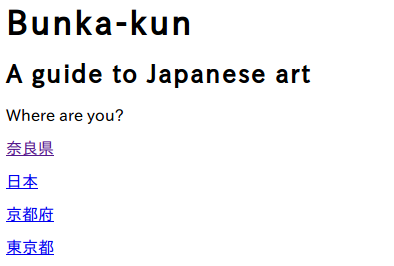
\includegraphics[width=\textwidth]{bunka1.png}
          \caption{Asking user for location}
          \label{fig:bunka1}
  \end{subfigure}
  \begin{subfigure}[b]{0.4\textwidth}
    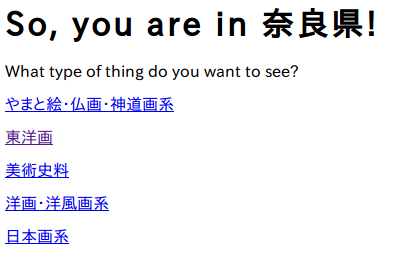
\includegraphics[width=\textwidth]{bunka2.png}
    \caption{Asking user for type of art} \label{fig:bunka2}
  \end{subfigure}\
  \vspace{10mm}
  \begin{subfigure}[b]{0.5\textwidth}
    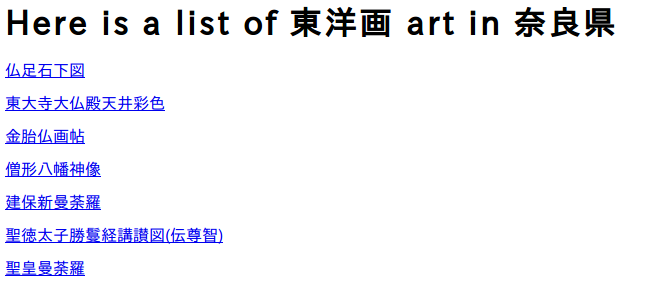
\includegraphics[width=\textwidth]{bunka3.png}
    \caption{Displaying a list of links to the LODAC pages for the matching artifacts}
    \label{fig:bunka3} 
  \end{subfigure}
\caption{The ``Bunka-kun'' art browser}
\label{fig:bunka} 
\end{figure}

\subsection{Querying the LODAC database} The site works by asking the user a series of questions and sending a SPARQL query to the LODAC server based on their answer.  The back-end code was written in Clojure \cite{clojure} and uses a domain specific language to form the SPARQL queries \cite{matz}, then rendering an HTML page using Hiccup \cite{hiccup} based on the LODAC endpoint's response.  

\section{Visualising the links between artists} The ``Bunka-kun'' art browser was an interesting way to find certain types of art in a certain location, but I was more interested in the artists themselves and the links between them. What would be a good way to visualise the communities of artists and the links between them? The next project was to create a force-directed graph visualisation that clustered together different kinds of artists, called `Artvis'.  

\subsection{Getting the data} The easiest way to find out information about the artists was to get their category information from DBPedia. This was done by first finding which artists existed in both DBPedia and LODAC, simply by comparing the strings of the artists' names. This resulted in a total of about 200 artists with entries in both DBPedia and LODAC. 

\subsection{Making a force-directed graph} 
\begin{figure} 
  \centering
  \begin{subfigure}[b]{0.9\textwidth} 
    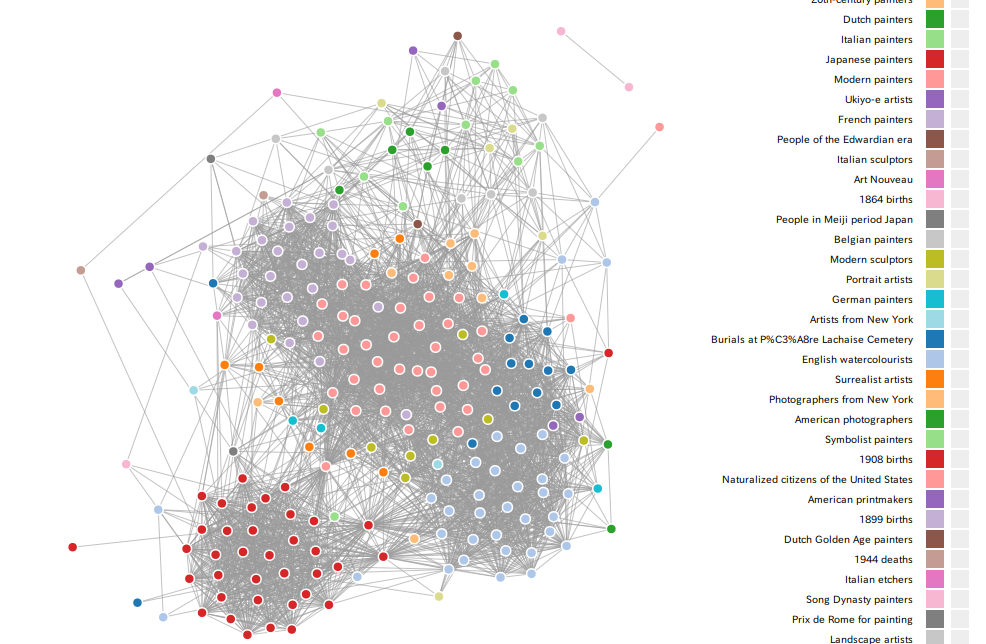
\includegraphics[width=\textwidth]{artvis1.png} 
    \caption{Showing all nodes on a graph. Hovering the mouse over a node shows the artist's name and main category.} 
    \label{fig:artvis1} 
  \end{subfigure}\\
  \vspace{10mm} \begin{subfigure}[b]{0.9\textwidth}
  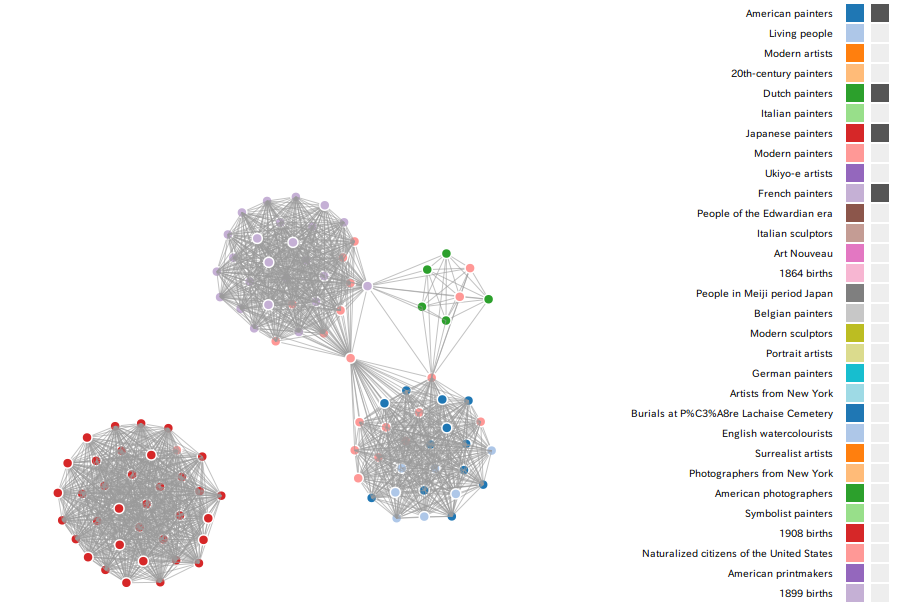
\includegraphics[width=\textwidth]{artvis2.png} 
  \caption{Artvis with the `American painters', `Dutch painters', `Japanese painters' and `French painters' categories selected.} 
  \label{fig:artvis2} 
\end{subfigure} 
\caption{The ``Artvis'' graph visualisation}
\label{fig:artvis} 
\end{figure} 

The next thing I made was a graph-based visualisation of the artists. The nodes of the graph were coloured and clustered according to the DBPedia category that each artist belonged to.  The data used was gathered by querying the DBPedia SPARQL endpoint based on artists that exist in the LODAC database. This was then compiled into a JSON data format to be read by the Javascript D3 (Data Driven Documents) visualisation library \cite{d3} for display on the site. 

Some custom code to filter the artists by category was then added.  The visualisation first shows all artists that it knows of. These artists are displayed as nodes on a force-directed graph, linked together if they share a category in the DBPedia database. This kind of visualisation naturally clusters the nodes together into communities that share the same categories.  Each node was assigned a colour based on the category it shares with the greatest number of other artists. For example, say an artist belongs to the three categories of Japanese painters, Impressionists and Sculptors. If there are more sculptor artists in the dataset than Japanese painters or Impressionists, then the artist's node is assigned the colour that corresponds to sculptors.  Subsets of artists can be selected by clicking on checkboxes next to a legend to the right of the visualisation.

In figure \ref{fig:artvis2}, the user has clicked on the `American painters', `Dutch painters', `Japanese painters' and `French painters' checkboxes, therefore only the artists that belong to these categories appear in the visualisation.

Hovering the mouse over an artist's node displays the name of the artist and their most popular category.

This type of visualisation is very convenient for seeing which artists bridge different communities. As shown in figure \ref{fig:artvis2}, one artist, Yves Tanguy, is connected to both French Painters and American Painters.

The visualisation is available online at \url{http://cblop.com/artvis}.

\section{Automatic taxonomy generation}
The main problem with the Artvis visualisation was that the categories of artists appeared as a big, arbitrarily-ordered list. This is not ideal for browsing through different types of artists. Ideally, the user would be able to browse through a hierarchical taxonomy of categories of artists, drilling down from vague categories such as `Japanese artists' down to more specific ones such as `Edo period Ukiyo-e painters'.

Unfortunately, such a taxonomy does not exist for Wikipedia's or DBPedia's artist categories. This was an opportunity to see if one could be formed automatically from available data.

\subsection{Gathering more data}
% talk about wikilinks and categories
% also: Japanese DBPedia, Keio ontology
For the Artvis visualisation, only artists from English DBPedia that also occurred in the LODAC ontology were used. This was a very small number of artists, only around 200.

In order to automatically create a taxonomy, more data from more artists would be required. I used the same basic string matching tools to link 172 artists from Japanese DBPedia, 280 from English DBPedia (using the sameAs attribute to find the Japanese equivalent from Japanese DBPedia) and 791 from Keio University's Wikipedia ontology at \cite{keio}.

\subsection{Heymann taxonomy generation algorithm}
\begin{figure}
        \centering
                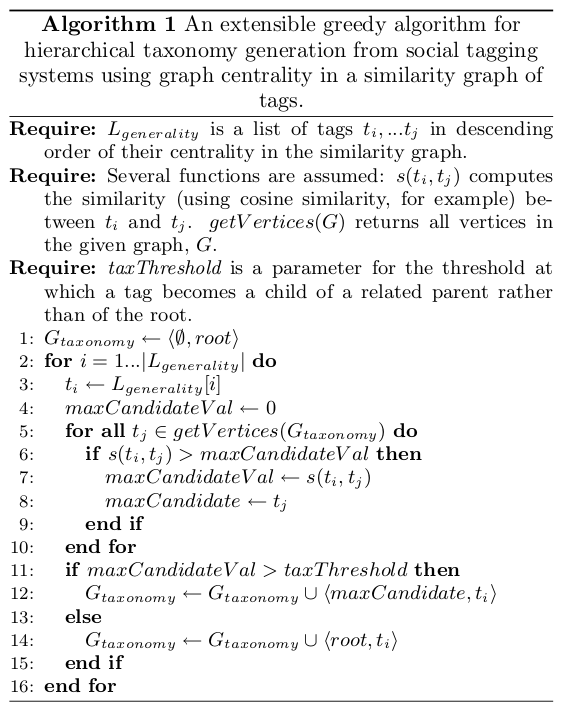
\includegraphics[width=0.7\textwidth]{algorithm.png}
\end{figure}

For the first attempt at taxonomy generation, I implemented a version of Heymann's automatic taxonomy generation algorithm \cite{heymann2006collaborative}. Algorithm 1 shows the pseudocode for this algorithm.

The algorithm requires some kind of way of computing the similarity between two tags. In my implementation, I used a very simple score. The score for each pair of tags is how many times they appear together in an artist's list of DBPedia categories.

An example visualisation of the generated taxonomy is shown in figure \ref{fig:taxon}. The full hierarchy can be browsed online at \url{http://cblop.com/tax_cat}.

% (description of how the algorithm works goes here)
\begin{figure}
        \centering
                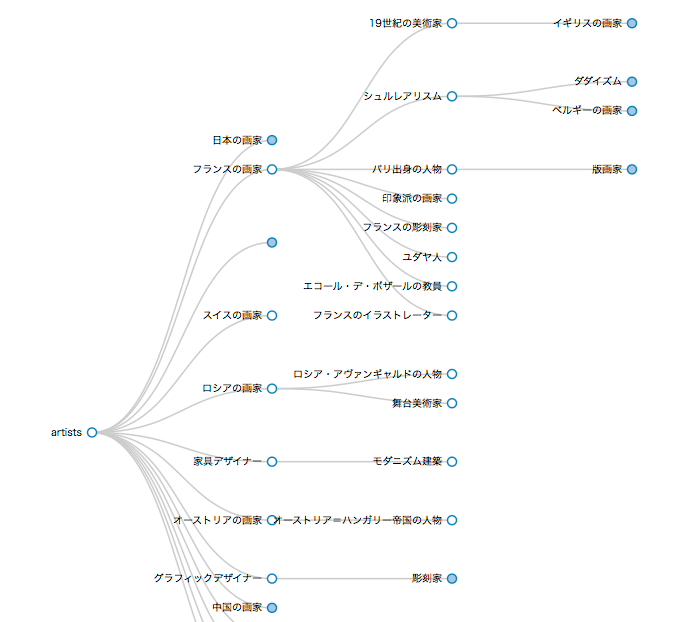
\includegraphics[width=0.9\textwidth]{taxon.png}
        \caption{Taxonomy generated by using Heymann's automatic taxonomy-generating algorithm}\label{fig:taxon}
\end{figure}

\subsection{Hierarchical clustering}
Next, I tried a more low-level approach using hierarchical clustering to group the artists together. Using this method, the taxonomy was derived by looking at the most common categories that belonged to each cluster of artists and putting those categories together within the taxonomy.

Although this does not provide a hierarchical taxonomy, it is possible to derive this kind of taxonomy by cutting off the tree at certain points.

The dendrogram in figure \ref{fig:dendro} shows the clustering of artists. The diagram is coloured to show how the artists are clustered at a reasonably low level, with a threshold value of 6. Looking at the artist names in the diagram, it is clear that the names of non-Japanese artists in Katakana are grouped together as one would expect.

\begin{figure}
        \centering
                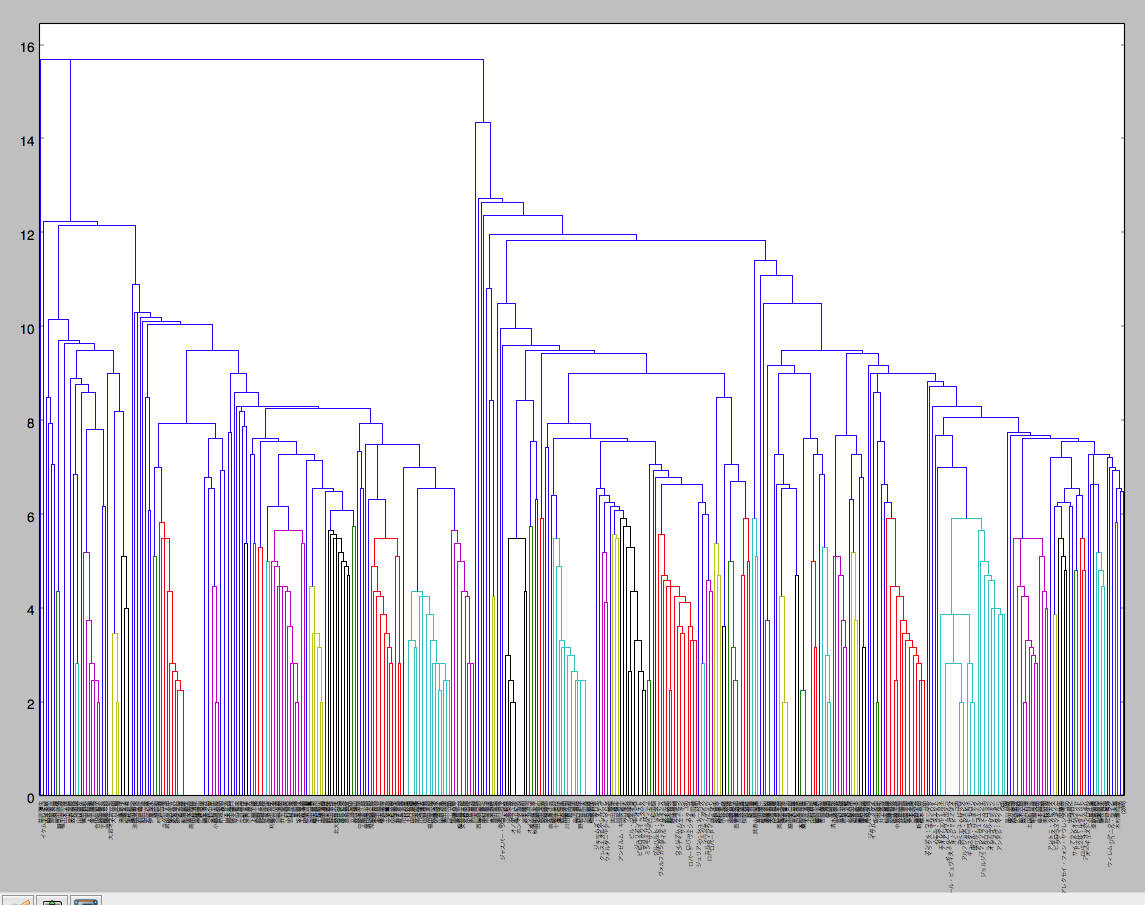
\includegraphics[width=0.9\textwidth]{dendro.png}
        \caption{Dendrogram of the hierarchical cluster of artists, coloured with a threshold value of 6}\label{fig:dendro}
\end{figure}

\section{Art browser app}
\begin{figure}
        \centering
                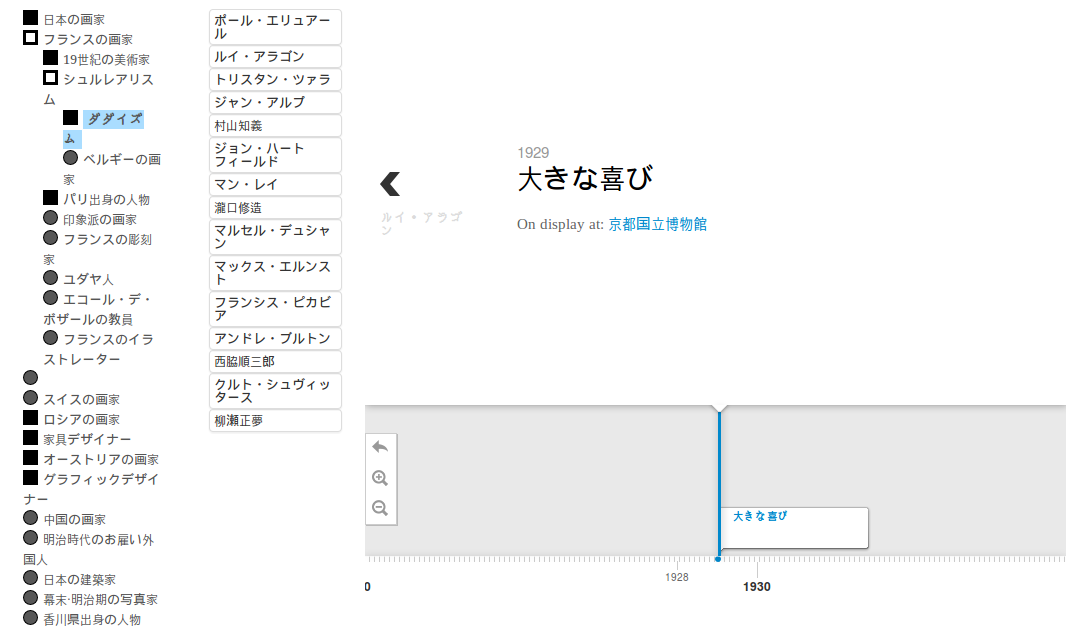
\includegraphics[width=0.9\textwidth]{timeline.png}
        \caption{Screenshot of the artist timeline browser}\label{fig:timeline}
\end{figure}
\subsection{Motivation}
For the newcomer to Japanese art, it is difficult to discover new artists. I wanted to make a system where a user could browse through a taxonomy of artists to find ones that they know and have the system recommend new artists based on their selection. They would also be able to see other artists in the same level on the taxonomy to find artists within the same genre as ones that they like.

Also, it would be good to see all the artworks for a given artist and which museums in Japan have them on display. I decided to show all the artworks on a timeline to do this. A user browses a list of artworks that are chronologically organised for each artist.

\subsection{Technology used}
Using the taxonomy generated using Heymann's algorithm, a tree of artist categories is shown on the right. I used the Angular.js Javascript library to allow realtime filtering of the artists based on the selected categories.

Once an artist is selected, their timeline of artworks appears on the right. I used the Timeline.js library to read in a JSON file for each artist that holds a list of their artworks along with the dates they were created and where they can be found in Japan.

A screenshot of the resulting application can be seen in figure \ref{fig:timeline}, and online at \url{http://cblop.com/timeline}.

\section{Conclusions and future work}
\subsection{Facet-based browsing}
Ideally, a better way of browsing throught the categories of artists would be used.

Although the hierarchies that were generated are informative, they are not enough on their own to facilitate a useful way of browsing through the artists. The problem is that the higher levels of the hierarchy tend to be nationalities. What if the user wants to find all impressionists, not just those that are French? Under the automatically generated taxonomy, this would not be possible.

With this in mind, a facet-based way of browsing through the artists should be explored. This would enable the user to browse taxonomies of artists based on (for example):
\begin{itemize}[noitemsep]
  \item Nationality
  \item Period
  \item Materials used
  \item Movement/genre
\end{itemize}

The user would be able to select one way of browsing the artists, then browse them based on the facet. Each facet wolud display a different taxonomy to the user.

Once the user clicks on a tag in the taxonomy, it is added to a list used to filter the artists that are displayed.

Also, a search feature should be added so that the user can simply type in the name of an artist or tag, and the esults would be displayed on the right.

\bibliographystyle{plain}
\bibliography{report}

\end{document}

